\chapter{Results}
\label{sec:ergebnisse}
This chapter explores the results obtained from simulations using greedy algorithms, considering scenarios with and without tasking. It also looks into the effects of various weighting schemes discussed in earlier chapters. The simulations produce output files named detections, tracklets, and ephemerides, 
containing essential details like detection ID, fabricated NORAD ID, epoch, Signal-to-Noise Ratio (SNR), orbital elements, and other relevant information. The figures and findings presented in this chapter are based on the data extracted from these output files, providing a detailed analysis of algorithmic 
performance, the impact of tasking, and the influence of different weighting schemes.\\

\section{Comparison}

\begin{figure}[h!]
	\centering
	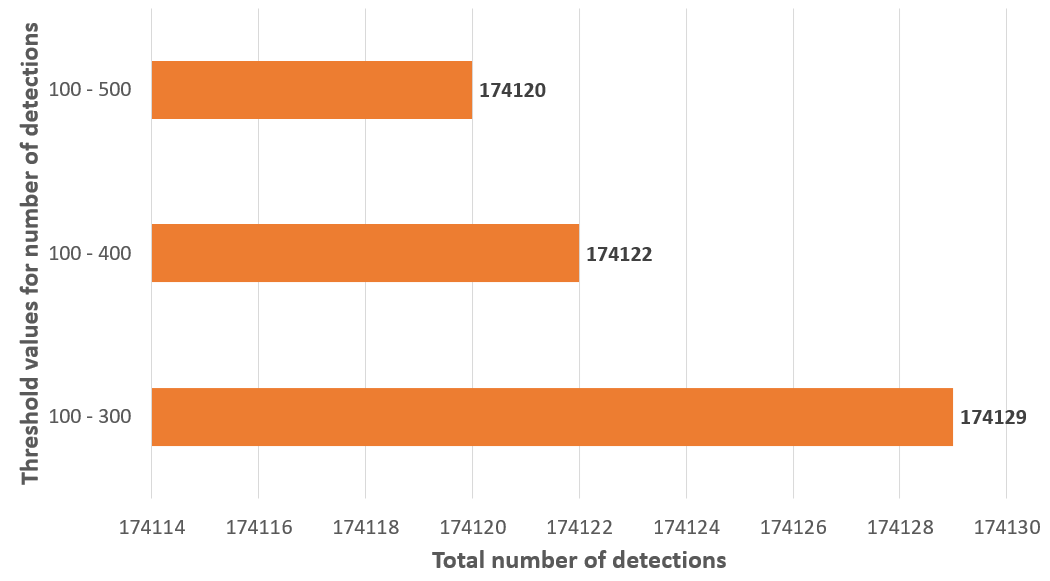
\includegraphics[width=0.8\textwidth]{Totdet_det.png}
	\caption{Total number of detections based on threshold values for number of detections of object}\label{fig:}
\end{figure}

\begin{figure}[h!]
	\centering
	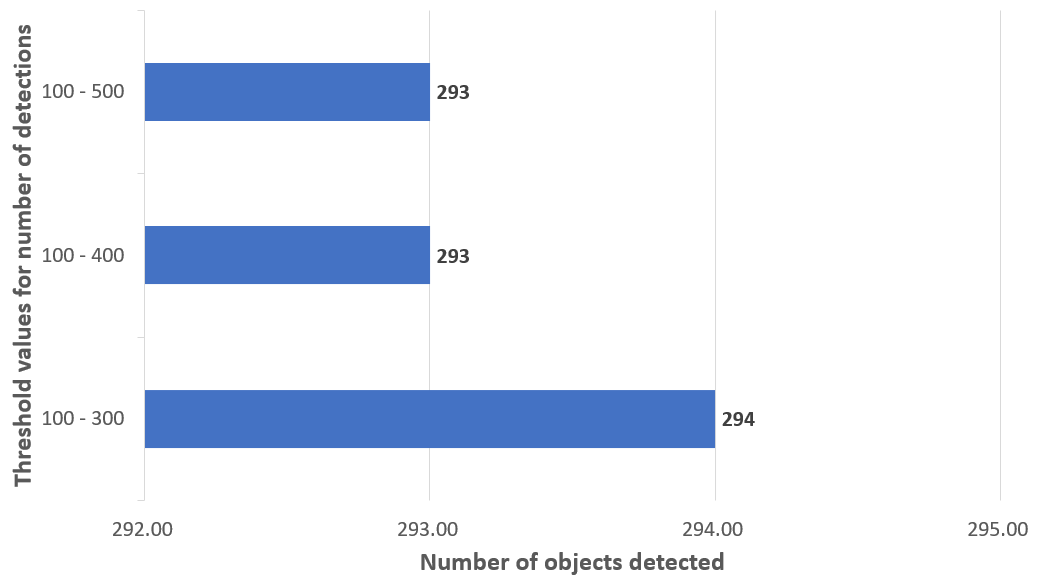
\includegraphics[width=0.8\textwidth]{UniqueObj_det.png}
	\caption{Total number of unique objects detected based on threshold values for number of detections of object}\label{fig:}
\end{figure}

\begin{figure}[h!]
	\centering
	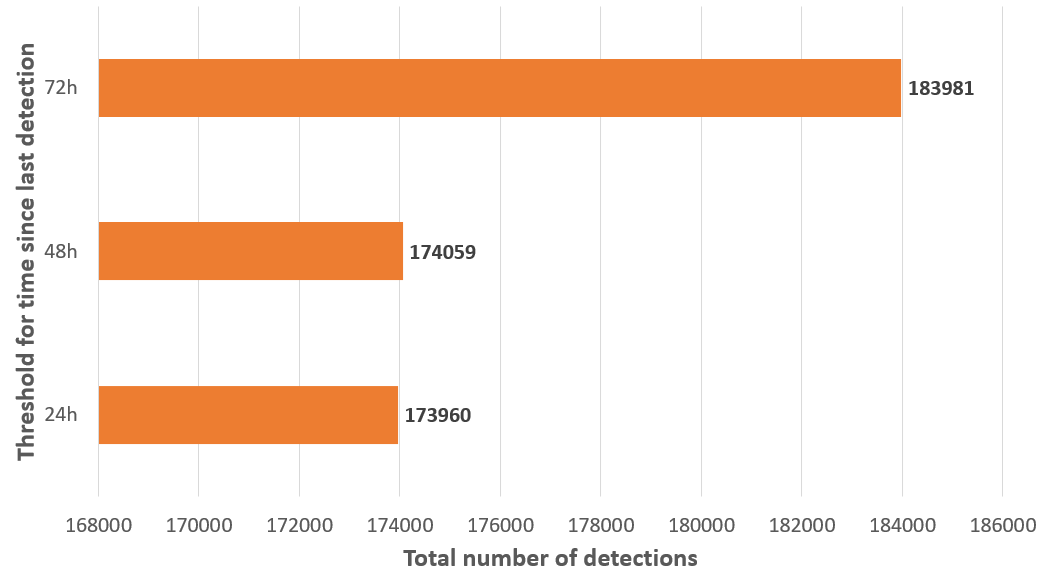
\includegraphics[width=0.8\textwidth]{Totdet_time.png}
	\caption{Total number of detections based on threshold values for time since last detection}\label{fig:}
\end{figure}


\begin{figure}[h!]
	\centering
	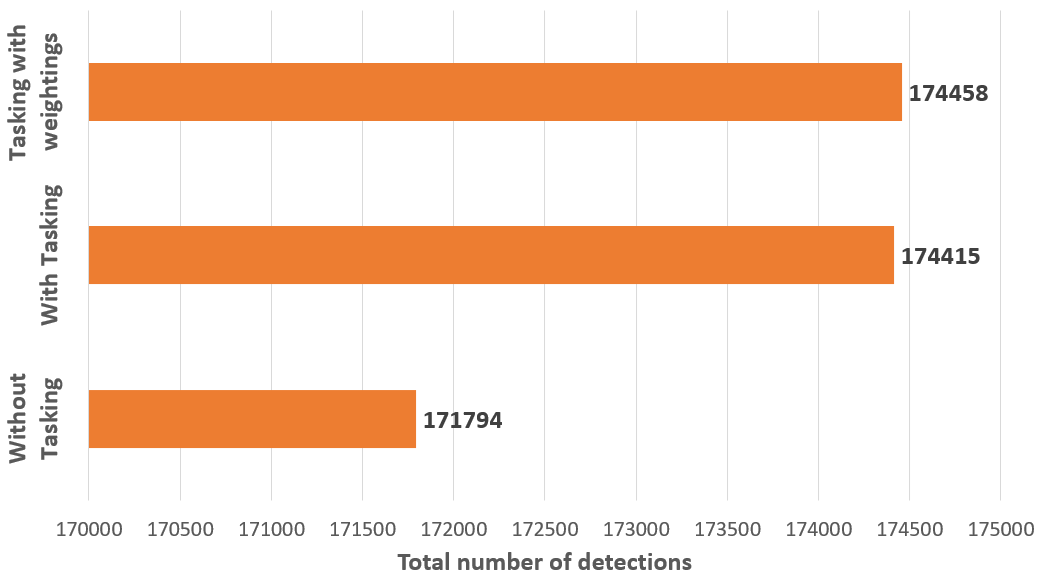
\includegraphics[width=0.8\textwidth]{numbofdet.png}
	\caption{Total number of detections compared with simulations without tasking, with tasking and tasking with Weightings}\label{fig:}
\end{figure}

\begin{figure}[h!]
	\centering
	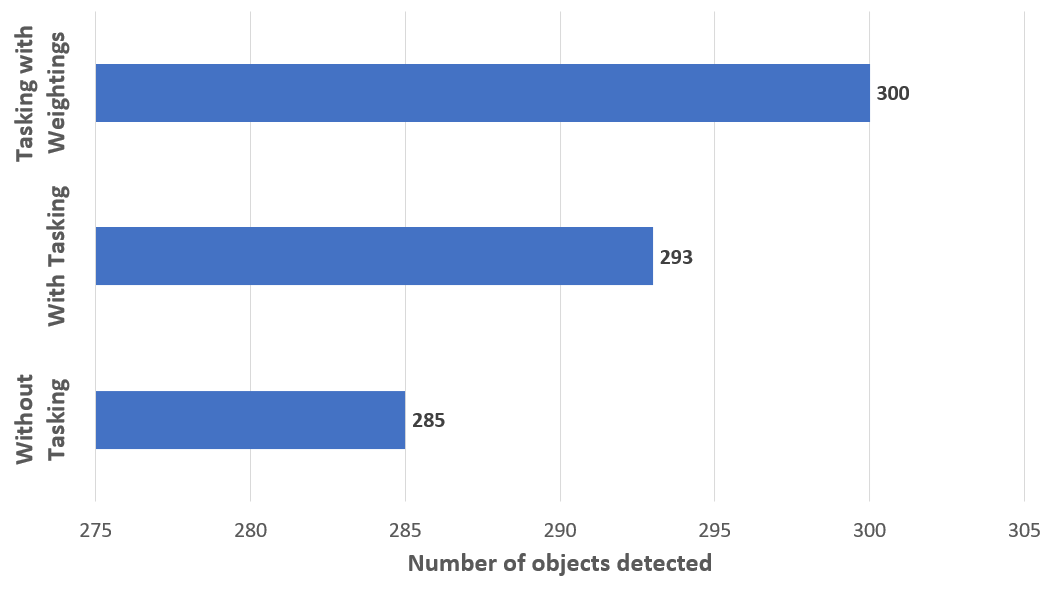
\includegraphics[width=0.8\textwidth]{numbofobj.png}
	\caption{Total number of objects compared with simulations without tasking, with tasking and tasking with Weightings}\label{fig:}
\end{figure}


\newpage
\section{Detections recorded in Horizontal coordinate system}

\begin{figure}[H]
	\centering
	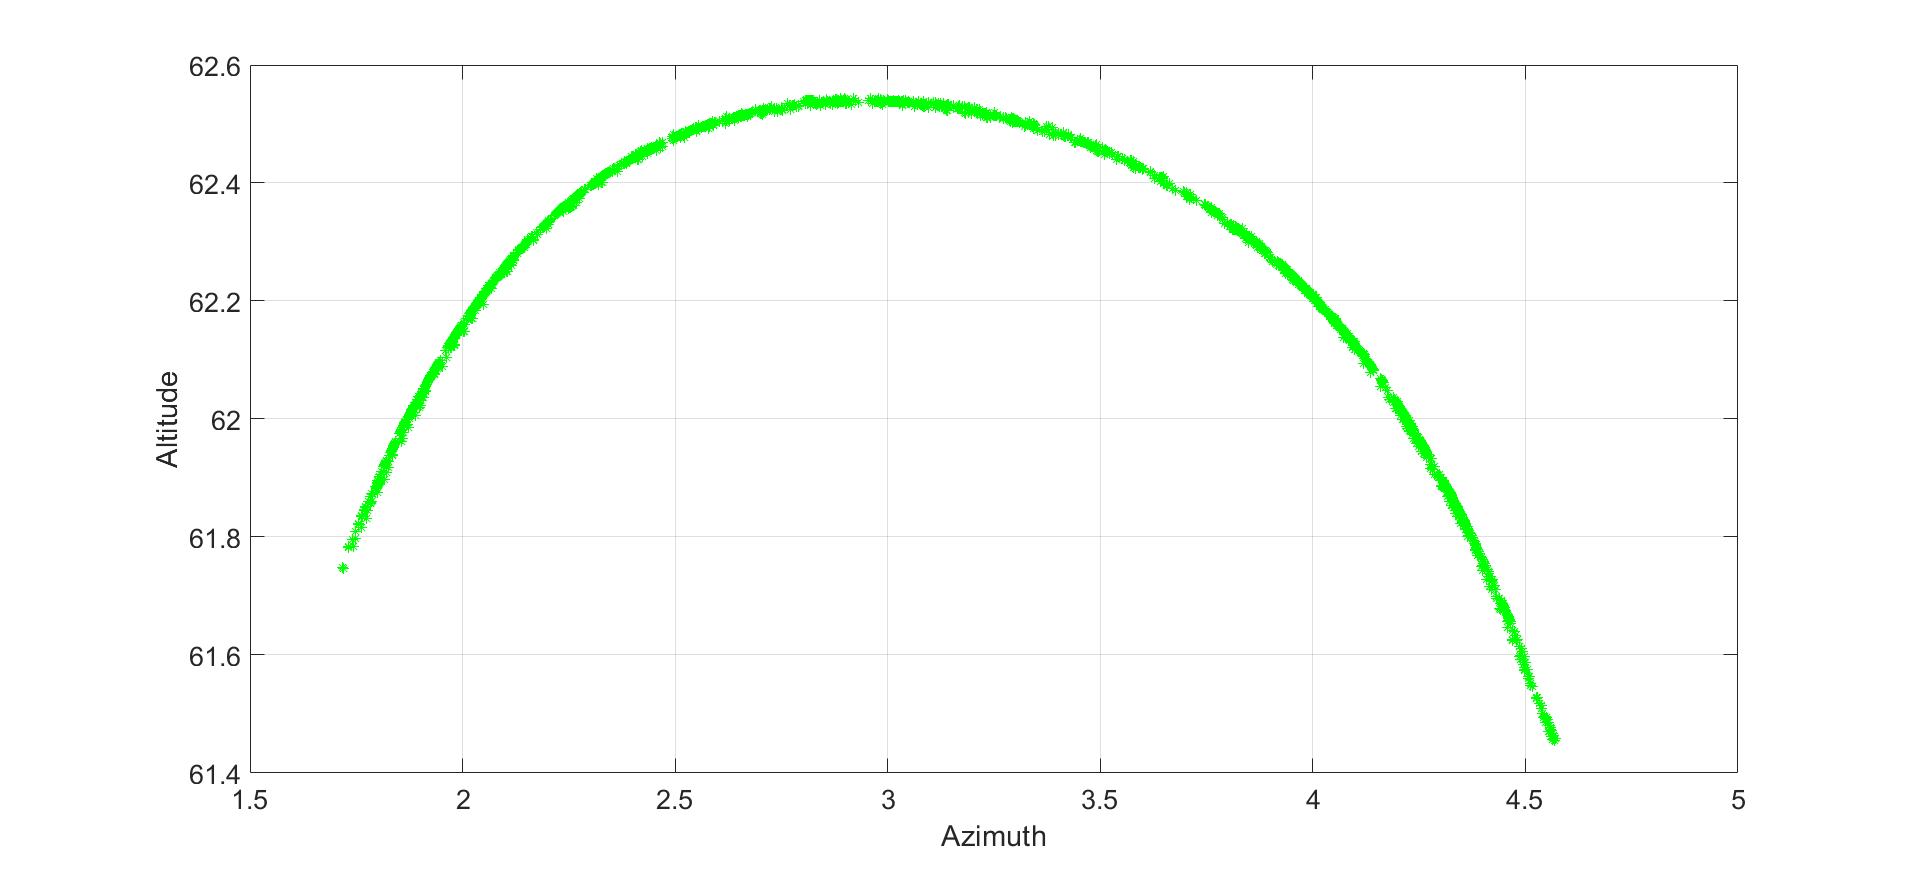
\includegraphics[width=0.9\textwidth]{AltvsAzHCS_1.png}
	\caption{Detections recorded by OGS in HCS (Without tasking)}\label{fig:}
\end{figure}


\begin{figure}[H]
	\centering
	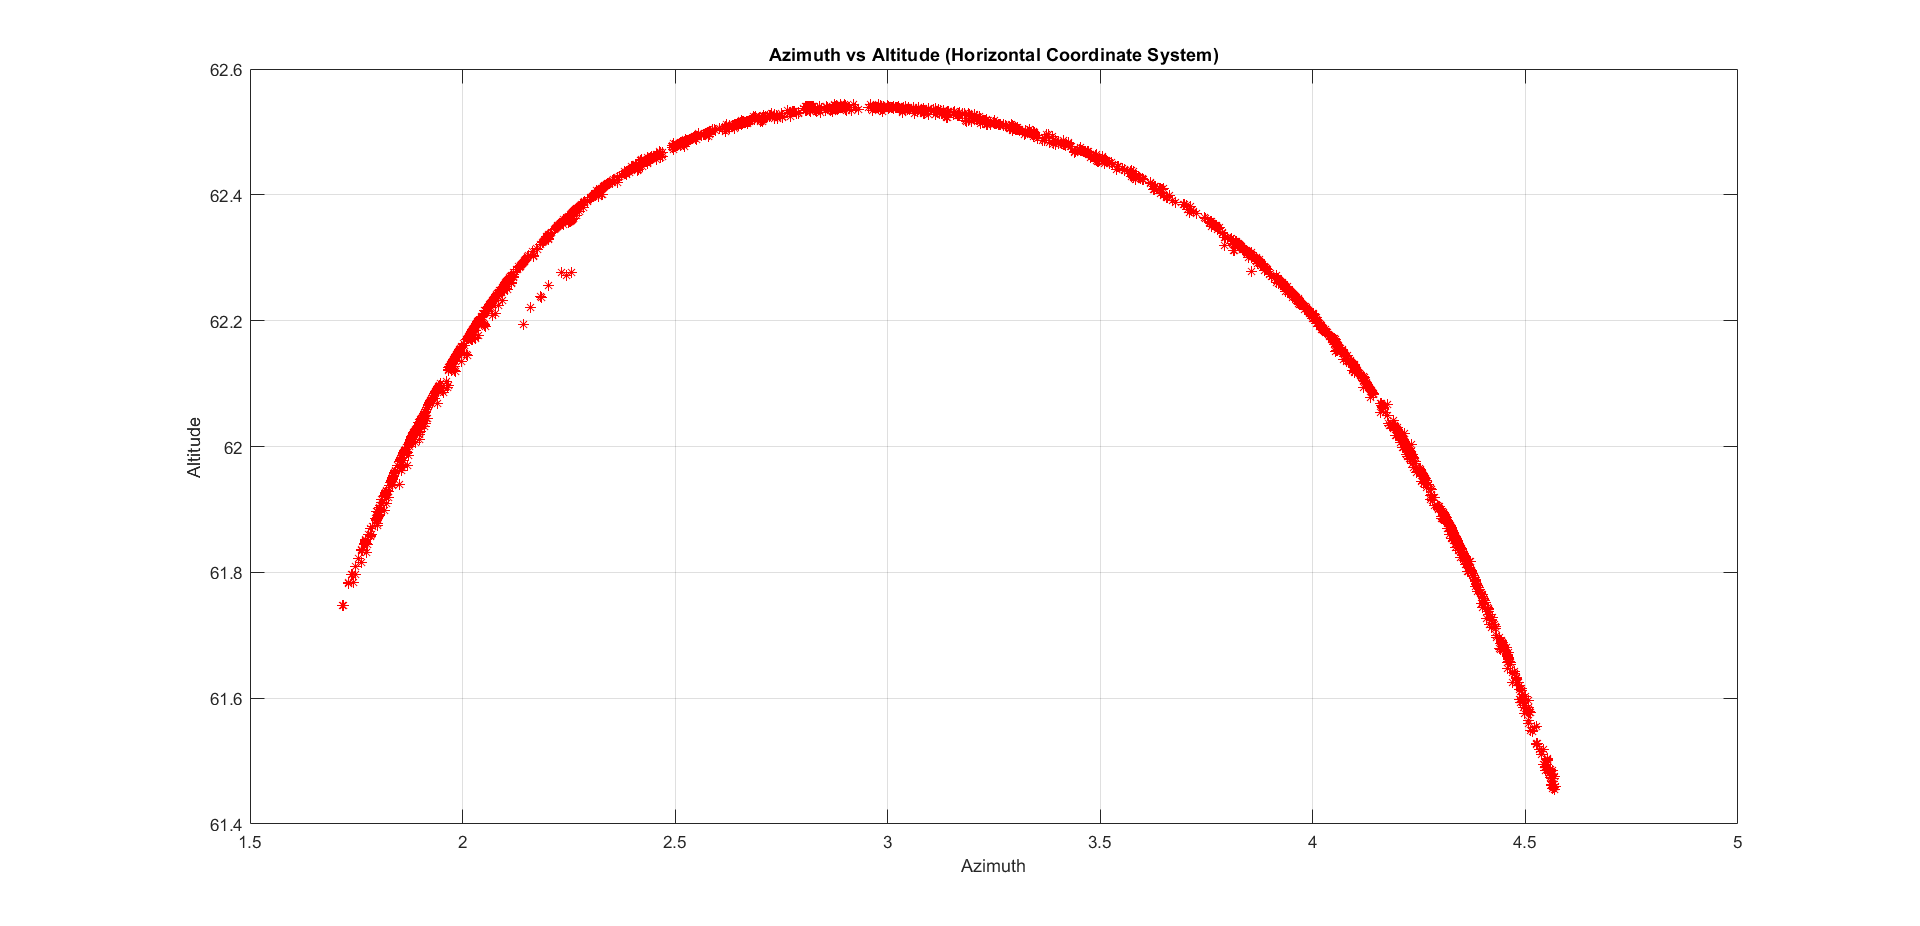
\includegraphics[width=0.9\textwidth]{AltvsAzHCS_8.png}
	\caption{Detections recorded by OGS in HCS (Tasking with Weightings)}\label{fig:}
\end{figure}

\begin{figure}[H]
	\centering
	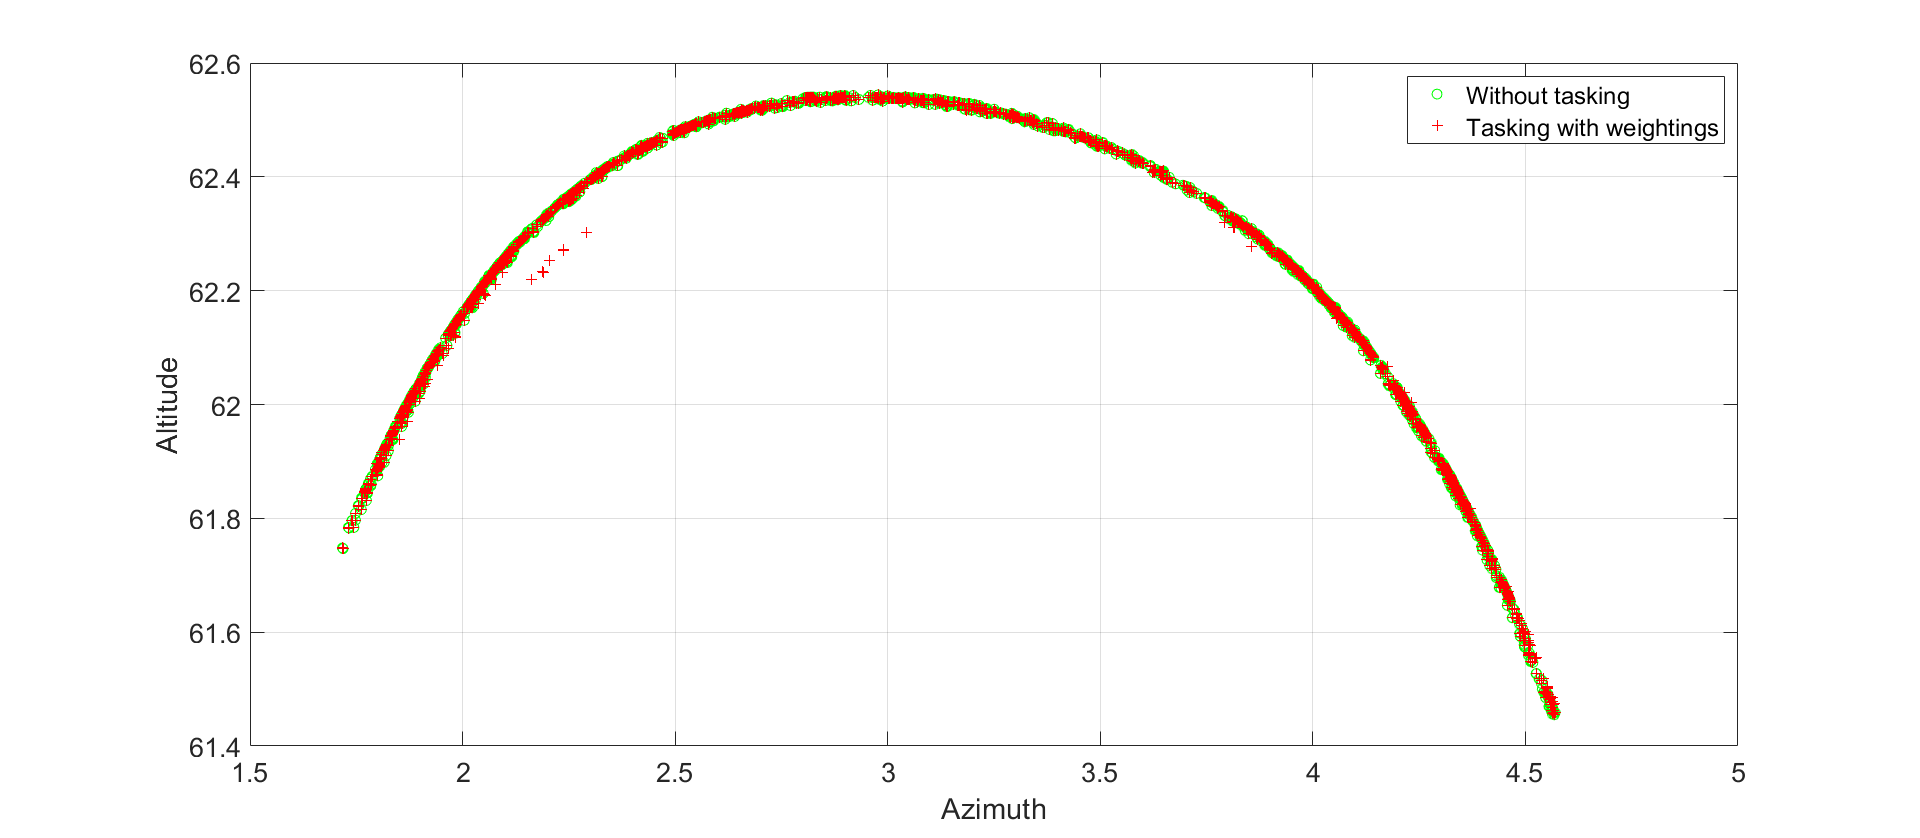
\includegraphics[width=0.9\textwidth]{AltvsAzHCS_comb.png}
	\caption{Detections recorded by OGS in HCS combined}\label{fig:}
\end{figure}


\newpage
\section{Detections recorded in Equatorial coordinate system}

\begin{figure}[h!]
	\centering
	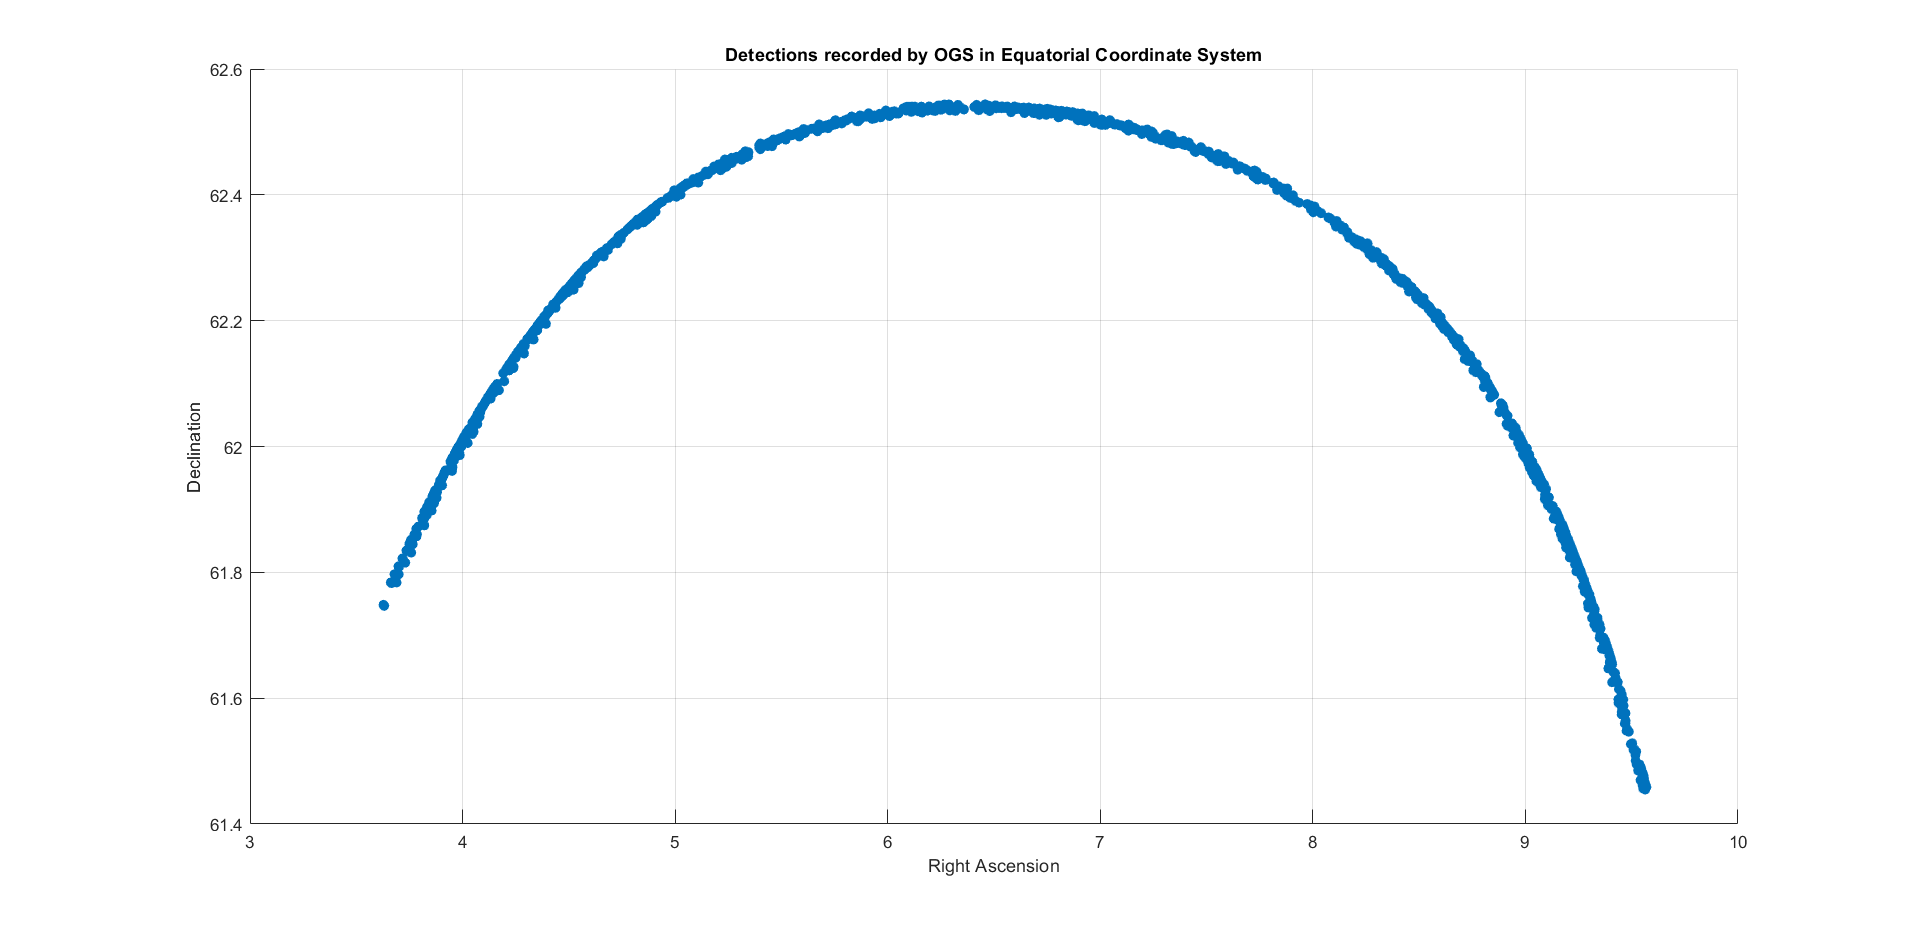
\includegraphics[width=0.9\textwidth]{DecvsRAECS_1.png}
	\caption{Detections recorded by OGS in ECS (Without tasking)}\label{fig:}
\end{figure}

\begin{figure}[h!]
	\centering
	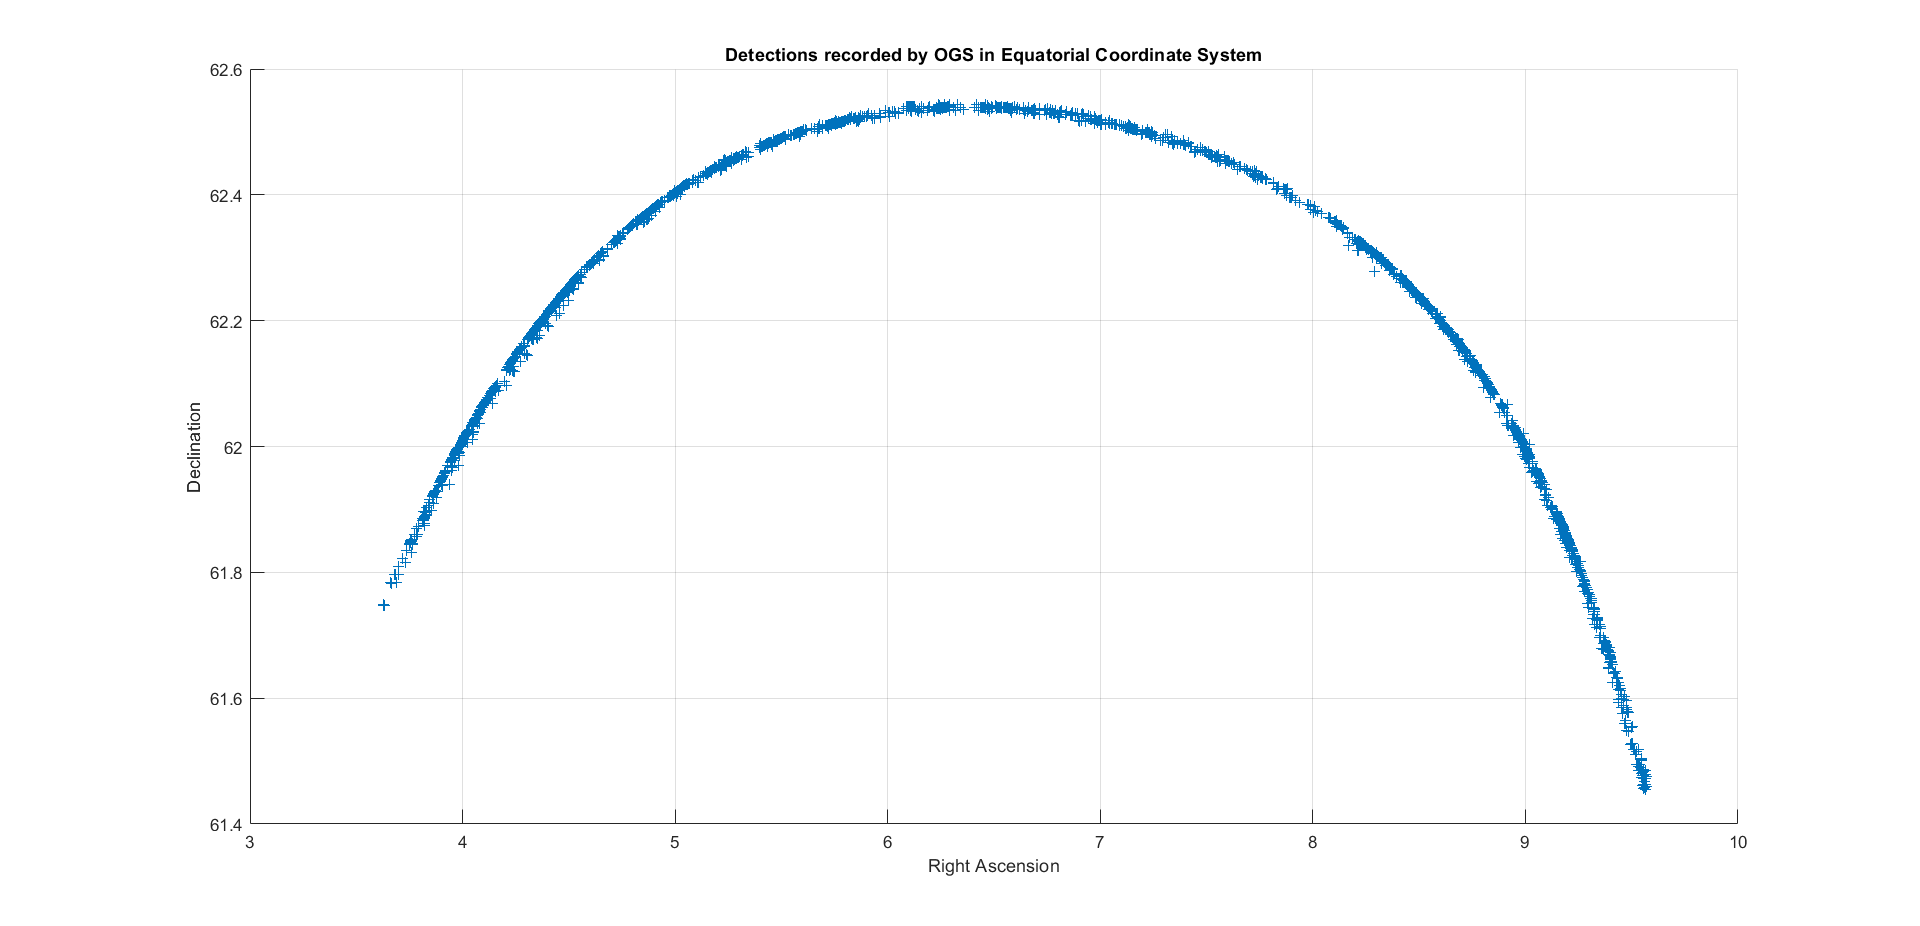
\includegraphics[width=0.9\textwidth]{DecvsRAECS_3.png}
	\caption{Detections recorded by OGS in ECS (Tasking with Weightings)}\label{fig:}
\end{figure}

\begin{figure}[h!]
	\centering
	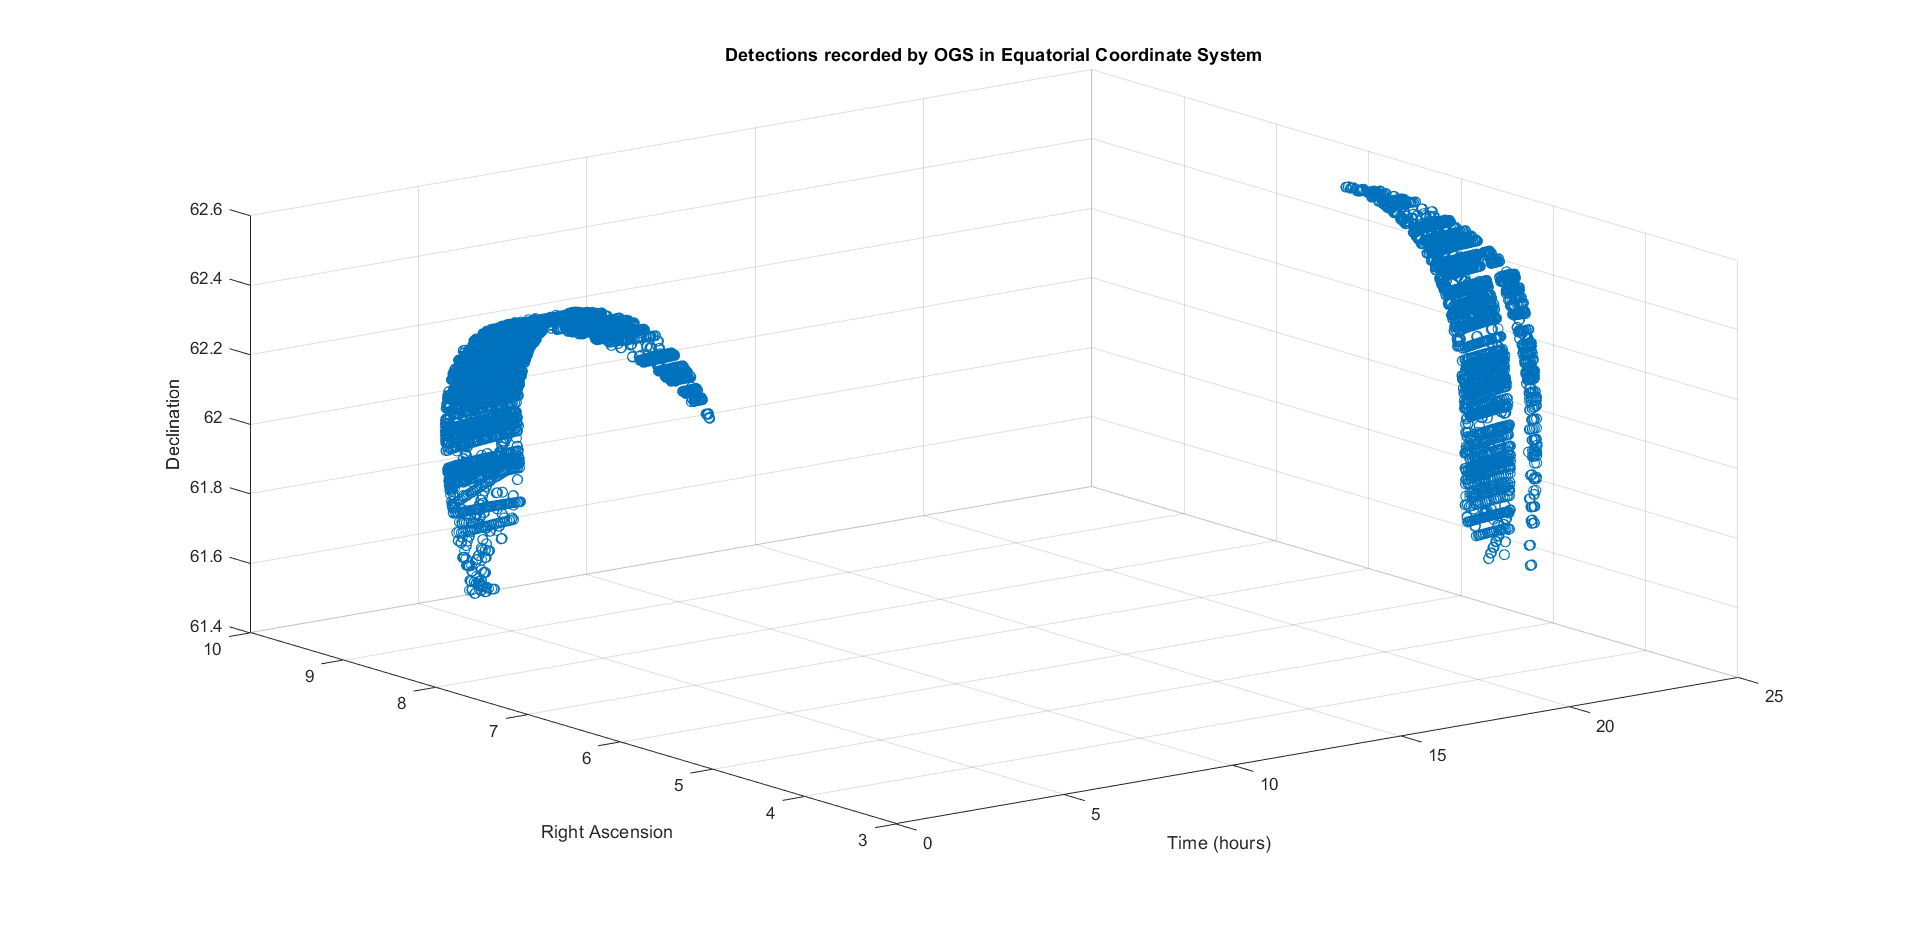
\includegraphics[width=0.9\textwidth]{DecvsRAvsTiECS_1.png}
	\caption{Detections recorded by OGS in ECS (Without tasking)}\label{fig:}
\end{figure}

\begin{figure}[h!]
	\centering
	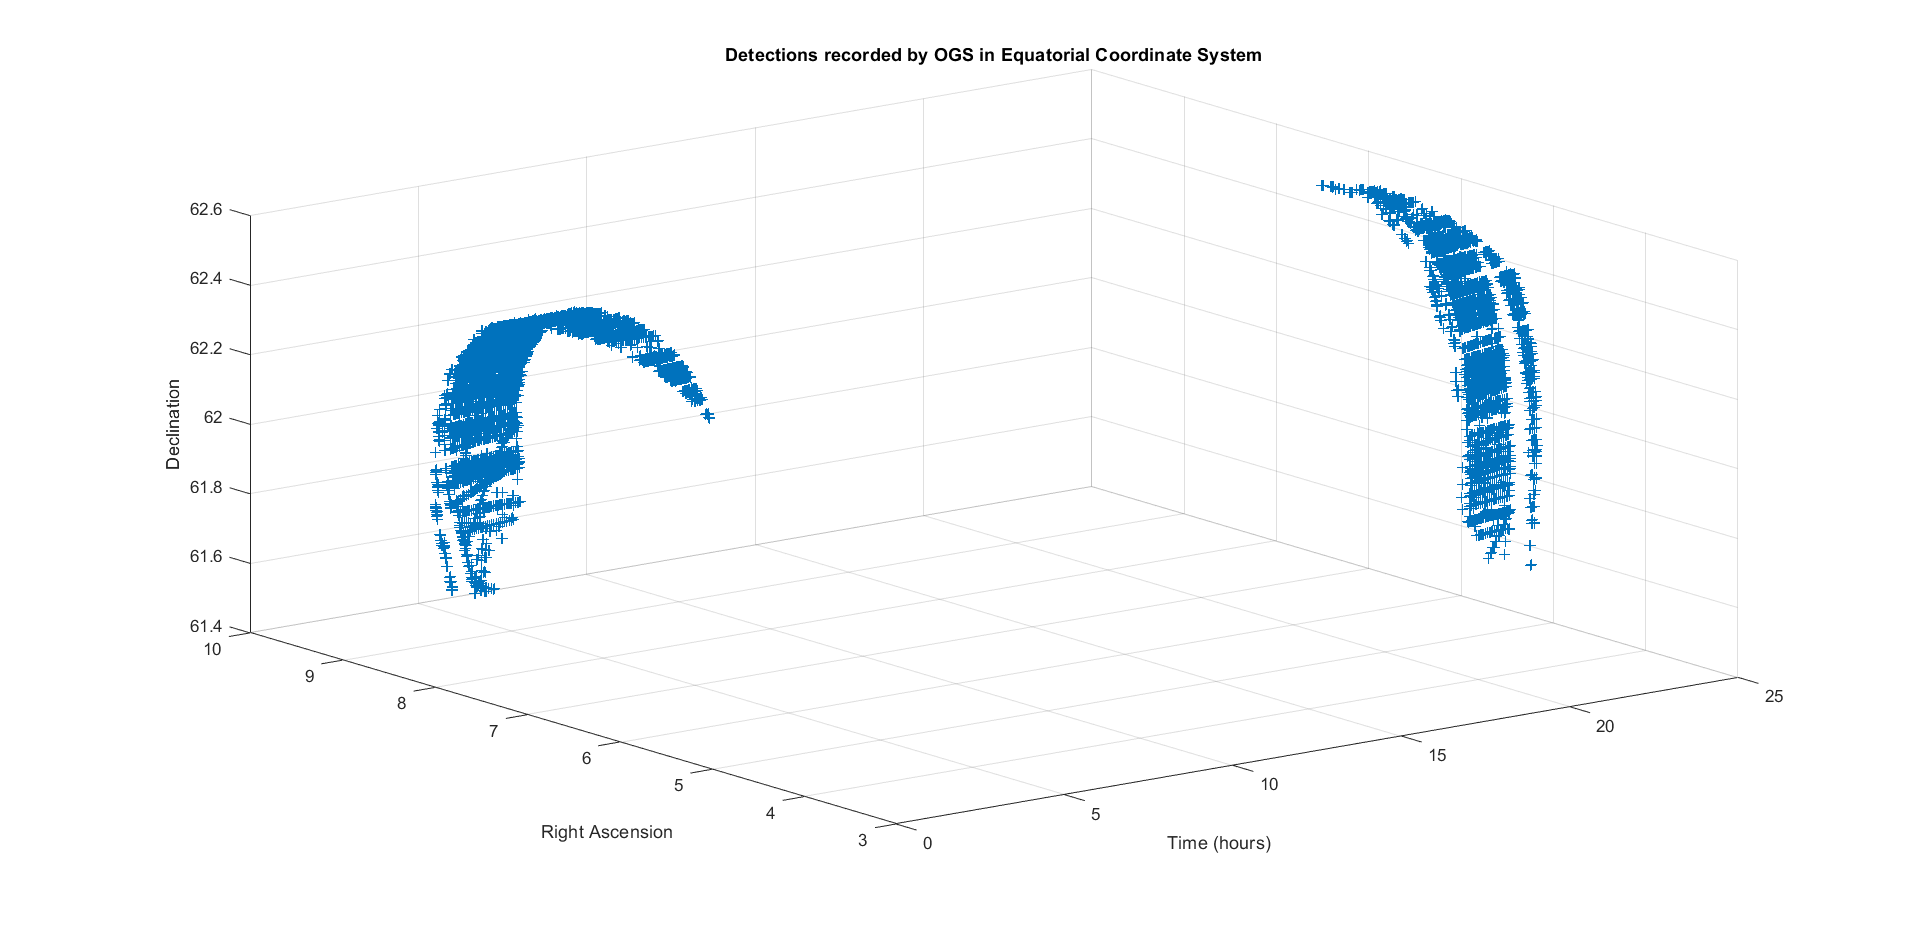
\includegraphics[width=0.9\textwidth]{DecvsRAvsTiECS_3.png}
	\caption{Detections recorded by OGS in ECS (Tasking with Weightings)}\label{fig:}
\end{figure}